% Original ROC/PR displays retained as supplementary figures.
\clearpage
\begin{figure}[p]\centering
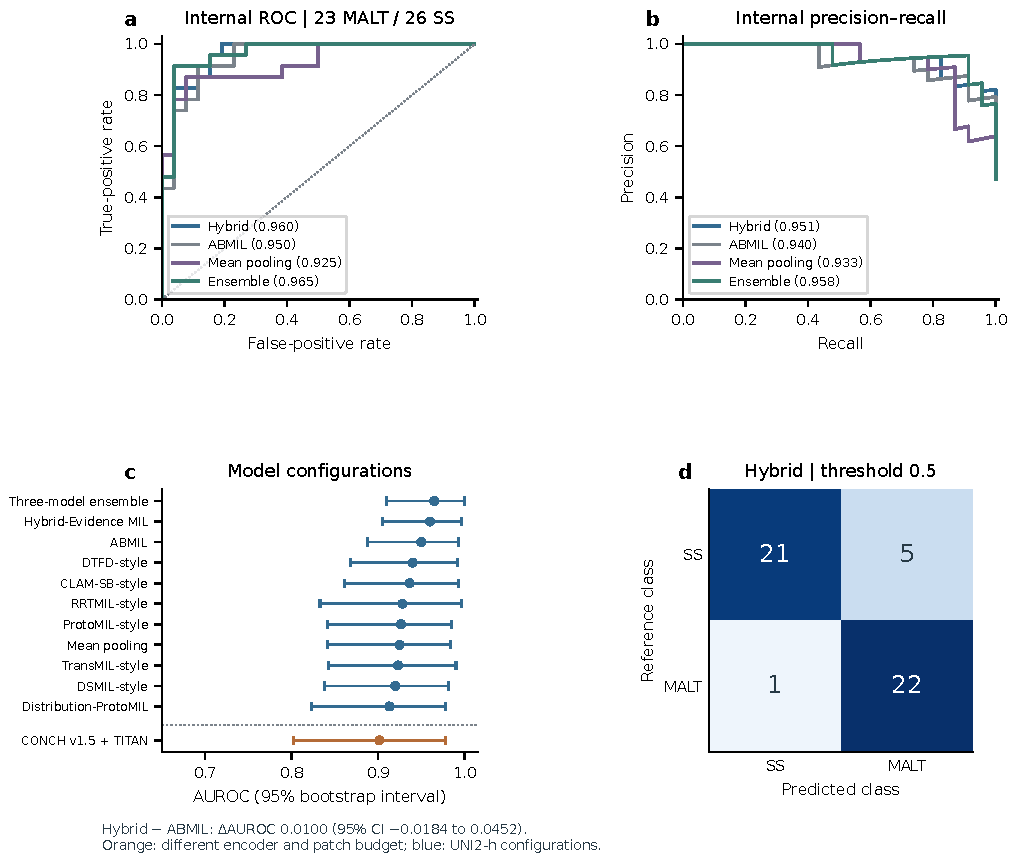
\includegraphics[width=\textwidth,height=.76\textheight,keepaspectratio]{figures/Figure_2_internal_performance.pdf}
\caption{\textbf{Internal validation discrimination and model configurations}. \textbf{a,b,} ROC and precision--recall curves on 49 WSIs (23 MALT and 26 SS). \textbf{c,} AUROC and 95\% intervals from 2,000 label-stratified WSI bootstrap samples of fixed predictions. Blue points use UNI2-h; the orange point uses a different encoder and patch budget. Simplified implementations retain their ``-style'' labels. The comparisons include complete implementations with different projection dimensions and training budgets. \textbf{d,} Hybrid confusion matrix at threshold 0.5. The 49 slides also selected checkpoints; intervals condition on fixed predictions and omit selection uncertainty. The paired Hybrid--ABMIL difference interval crosses zero. Source data are provided in internal\_model\_metrics.csv, paired\_model\_comparisons.csv and model-specific prediction tables.}\label{fig:S5}
\end{figure}

\clearpage
\begin{figure}[p]\centering
\fbox{\begin{minipage}[c][35mm][c]{.88\textwidth}\centering
\textbf{Omitted from this public repository copy}\\[6pt]
This figure contains tissue images or individual-slide observations.\\
The complete figure is retained in the local manuscript archive.
\end{minipage}}
\caption{\textbf{External performance and archive-tag composition}. \textbf{a,b,} ROC and precision--recall curves for four frozen model checkpoints on the same 168 WSIs (152 MALT and 16 SS), using identical reference bags for each slide. Legend values indicate AUROC and average precision, respectively. These compare complete implementations. The dotted PR reference is the MALT fraction. \textbf{c,} Confusion matrix at threshold 0.5. \textbf{d,} Individual uncalibrated model scores by diagnostic group and archive stain tag. Counts indicate correct predictions divided by group size; black marks show medians. Jitter separates points only. H\&E-like, IHC/special and HE-archive labels are provisional archive descriptors, not pathology-confirmed stains. Single-class groups have no within-group AUROC. Source data are provided in external\_final\_predictions.csv, external\_archive\_tag\_counts.csv and reference\_predictions.csv.}\label{fig:S6}
\end{figure}

\clearpage
\begin{figure}[p]\centering
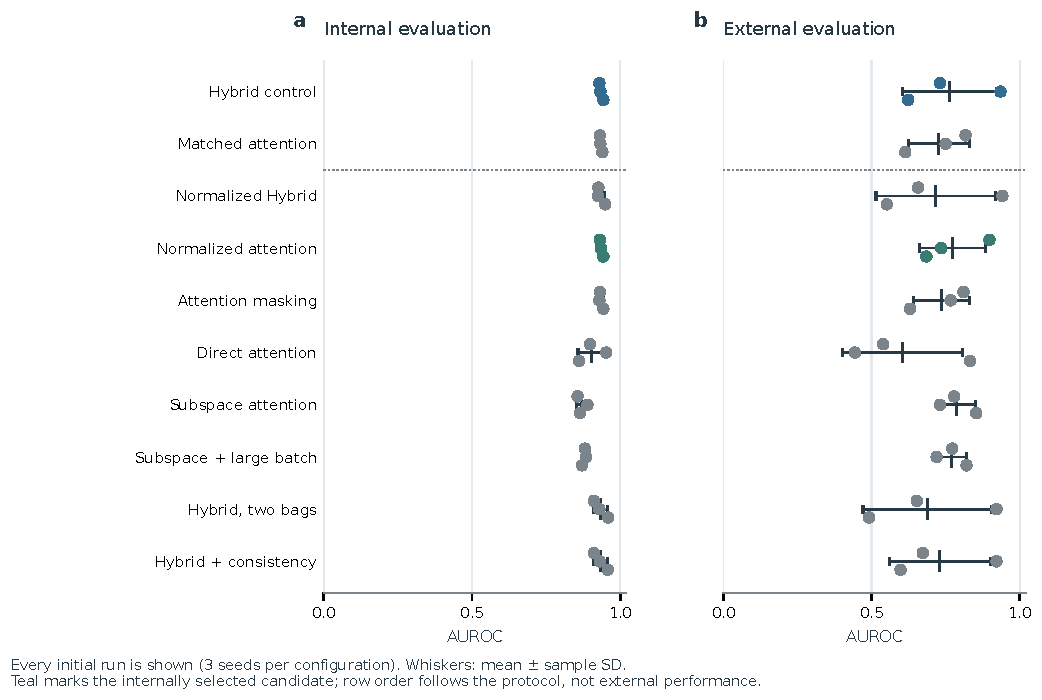
\includegraphics[width=\textwidth]{figures/Supplementary_Figure_S7_screening.pdf}
\caption{\textbf{All configurations in the bounded three-seed screen}. \textbf{a,b,} Internal and external AUROC for seeds 17, 29 and 43 in each of ten configurations. Every dot is one training run evaluated on the fixed cohort; horizontal ticks and whiskers indicate means and sample standard deviations, not confidence intervals. Controls are separated from the eight candidates by a dotted line. Teal marks normalized attention, selected using mean internal AUROC; the row order follows the protocol and is not ranked by external outcomes. The same 49 internal WSIs selected epochs, and the 168 external WSIs had been examined during prior development. Repeated control runs are not independent clinical replications. Full results are in Supplementary Table S16. Source data: run\_metrics\_verified.csv.}\label{fig:S7}
\end{figure}

\clearpage
\begin{figure}[p]\centering
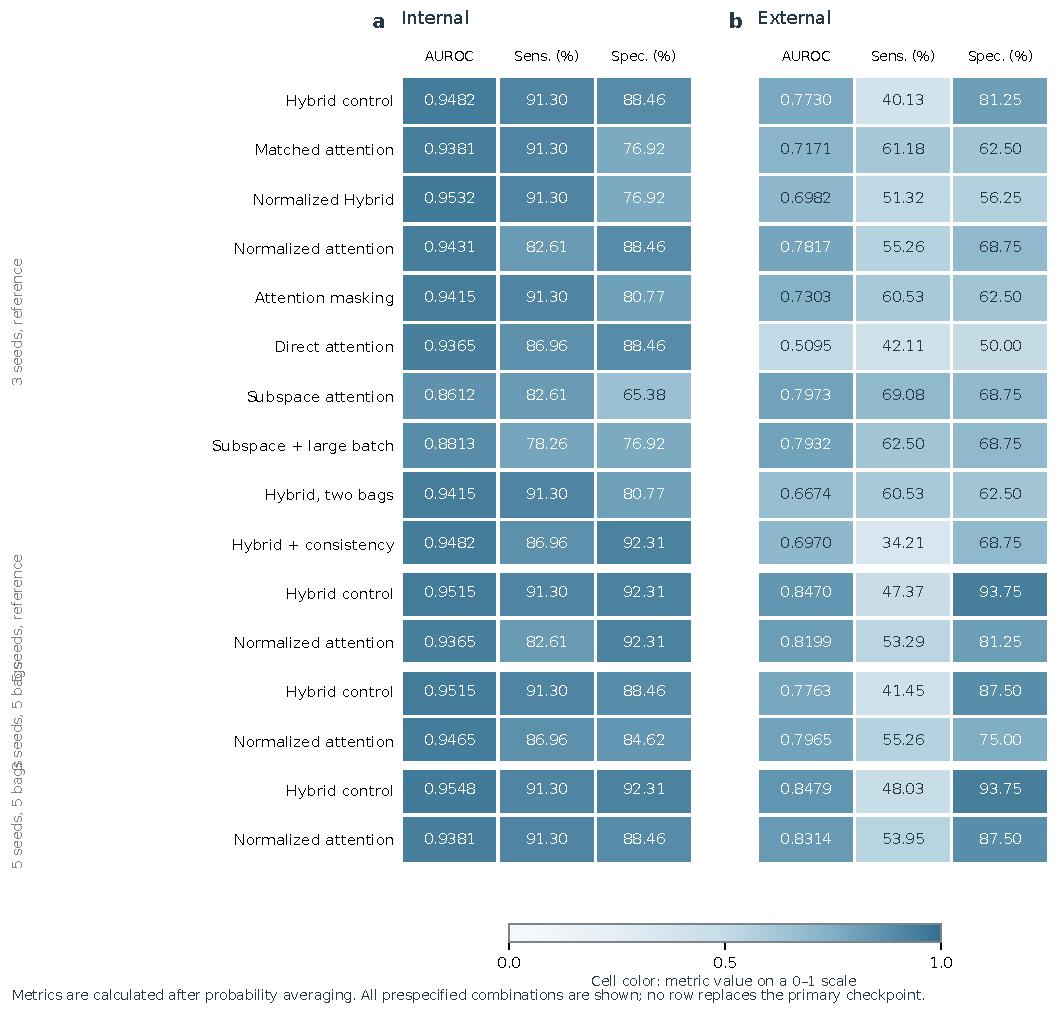
\includegraphics[width=\textwidth,height=.73\textheight,keepaspectratio]{figures/Supplementary_Figure_S8_aggregation.pdf}
\caption{\textbf{Prespecified probability-aggregation profiles}. \textbf{a,b,} Internal and external results for all sixteen configuration/aggregation combinations in Supplementary Table S19. Three seeds are 17/29/43; five seeds additionally include 59/71. Reference denotes the fixed 512-row reference bag; five-bag rules average five additional bags within each seed before averaging across seeds. AUROC is unitless; sensitivity and specificity are percentages at 0.5. Colors use a common 0--1 scale. Metrics are calculated from averaged probabilities rather than averaged across seed-level metrics. These are secondary analyses on reused evaluation material; no row replaces the historical primary checkpoint. The separate additional-two-seed summaries remain in the numerical archive. Source data: ensemble\_metrics.csv.}\label{fig:S8}
\end{figure}
